\chapter{Opis implementacji}
\label{ImplementationChapter}
System stworzony na potrzebę realizacji niniejszej pracy magisterskiej można podzielić na dwa moduły, zgodnie z opisem architektury zamieszczonym w sekcji \ref{SoftwareArchSection}:
\begin{enumerate*}
\item Środowisko Uczenia - stworzone w silniku Unity i odpowiedzialne za symulowanie wirtualnego środowiska, po którym przemieszcza się inteligentny agent.
\item Narzędzie \texttt{mlagents\_learn} - wchodzi w skład frameworka \textit{Unity ML-Agents} (por. \ref{UnityMlSection}) i odpowiada za trening sieci konwolucyjnych. Jest procesem niezależnym od silnika Unity, a komunikacja ze Środowiskiem Uczenia odbywa się poprzez specjalny mechanizm, którego implementacja pochodzi z tego samego frameworka.
\end{enumerate*}

W dalszej części rozdziału znajduje się szczegółowy opis każdego z modułów.

\section{Środowisko Uczenia}
Jest typowym projektem stworzonym na silniku Unity, a w jego skład wchodzi wiele katalogów i plików. W tej pracy skupię swoją uwagę na opisaniu jedynie najważniejszych elementów potrzebnych do zrozumienia aplikacji, zaś resztę informacji można pozyskać posiłkując się dokumentacją silnika, która jest bardzo dobrym źródłem wiedzy o tym narzędziu.

\subsection{Wykorzystane assety}
Assety to reużywalne komponenty, przeznaczone do wykorzystywania w projektach uruchamianych na silniku Unity. Assety mogą być zasobami jakiegokolwiek typu, począwszy od modeli 3D i plików audio, a skończywszy na skryptach języka C\#. W ramach silnika Unity udostępniana jest specjalna usługa o nazwie \textit{Unity Asset Store} \cite{unity:assetStore}, która zapewnia dostęp do darmowych i płatnych assetów.

W realizowanym projekcie jest wykorzystywanych kilka paczek assetów, lecz najważniejsze z nich są dwa: \textbf{Environmental Race Track Pack} oraz \textbf{Vehicle Physics Pro}, którego dokładny opis zamieściłem w sekcji \ref{VppSection}.

\subsubsection{Environmental Race Track Pack}
Darmowa paczka, w skład której wchodzą cztery odmienne tory wyścigowe złożone z relatywnie małej liczby trójkątów \cite{unityAssets:envRaceTrackPack}:
\vspace{-0.5cm}
\begin{itemize*}
\item ,,\textit{Coastal Race Track}'' - tor nadbrzeżny,
\item ,,\textit{F1 Race Track}'' - tor Formuły 1,
\item ,,\textit{Racing Oval}'' - tor w kształcie owalnym,
\item ,,\textit{Figure 8 Track}'' - tor w kształcie ósemki.
\end{itemize*}
Na potrzeby implementacji systemu wykorzystałem dwa tory z tej paczki, co dokładniej jest opisane w sekcji \ref{RaceTracksSection}.

\subsubsection{Vehicle Physics Pro}
Dokładny opis tego zestawu został zamieszczony w sekcji \ref{VppSection}, tutaj natomiast wspomnę o najważniejszym z wykorzystanych assetów, czyli samochodzie \textbf{Sport Coupe}. Jest to dokładnie odwzorowany model 3D samochodu sportowego, posiadający skonfigurowaną fizykę jazdy. \textbf{Sport Coupe} jest jednym z dwóch skonfigurowanych modeli samochodów, dołączanych do zestawu Vehicle Physics Pro. Drugim z nich jest \textbf{JPickup}, czyli model samochodu typu pickup. Obydwa modele zostały zaprezentowane na rysunku \ref{VppCarModels}. \\

\begin{figure}[h]
\begin{center}
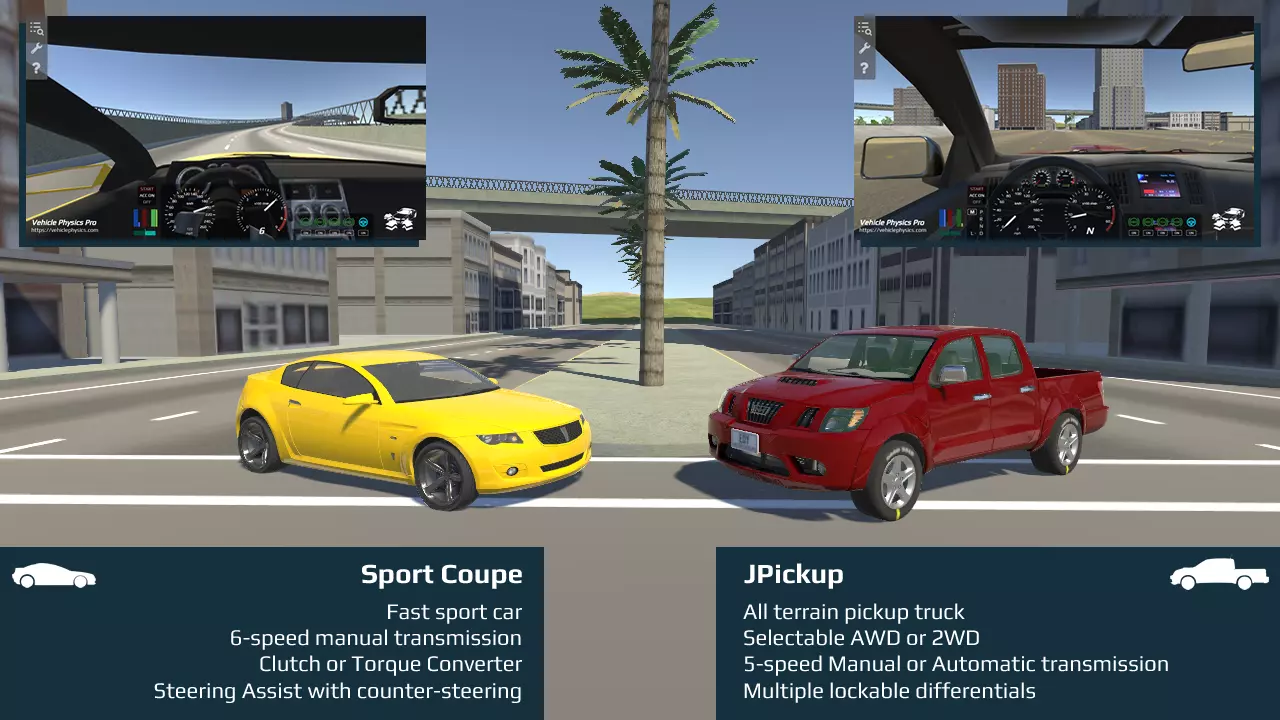
\includegraphics[width=14cm]{resources/figures/vpp-car-models.png}
\caption{Modele samochodów dostarczane w pakiecie Vehicle Physics Pro}
\source{https://assetstore.unity.com/packages/tools/physics/vehicle-physics-pro-community-edition-153556}
\label{VppCarModels}
\end{center}
\end{figure}

\newpage
\subsection{Tory wyścigowe}
\label{RaceTracksSection}
Na potrzeby implementacji systemu wybrałem dwa tory z pakietu \textbf{Environmental Race Track Pack}: ,,\textit{Figure 8 Track}'' oraz ,,\textit{Coastal Race Track}''. Tory uległy delikatnym modyfikacjom, polegającym przede wszystkim na usunięciu niepotrzebnych elementów sceny oraz zmianie jej oświetlenia. Widok torów z lotu ptaka został uwieczniony na rysunku \ref{RaceTracksFig}. \\

\begin{figure}[h]
\begin{center}
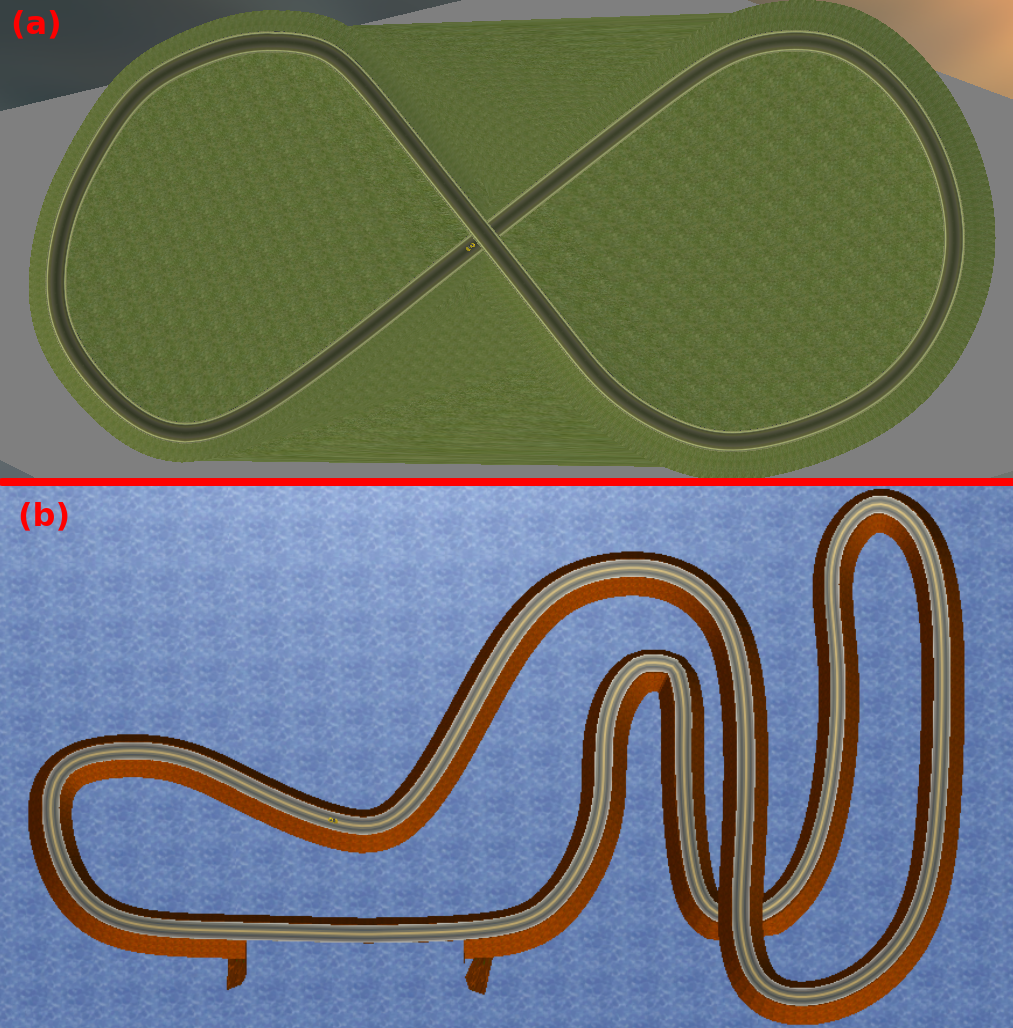
\includegraphics[width=14.5cm]{resources/figures/race_tracks_marked.png}
\caption{Tory wyścigowe wykorzystane w projekcie.}
\vspace*{-0.3cm}
\caption*{(a) Tor nr 1 - zmodyfikowany ,,\textit{Figure 8 Track}''}
\vspace*{-0.3cm}
\caption*{(b) Tor nr 2 - zmodyfikowany ,,\textit{Coastal Race Track}''}
\label{RaceTracksFig}
\end{center}
\end{figure}

\vspace{-0.5cm}
Tory różnią się od siebie przede wszystkim poziomem trudności - tor nr 2 wymaga od kierowcy znacznie większych umiejętności, ponieważ zakręty są bardziej zróżnicowane.

\subsection{Konfiguracja sceny Unity}
\section{Narzędzie mlagents\_learn}